\chapter{Calcium waves from IP3R}
\label{chap:calcium_waves_IP3R}

The two major discoveries in early studies of cytoplasmic calcium were:
sperms activate medaka eggs through a giant calcium wave (or calcium tsunami)
\citep{gilkey1978}, and increasing in concentrations of certain hormones can
induces increasingly frequent, periodic calcium oscillation in isolated
hepatocytes \citep{woods1986, woods1987}. 

The two pathways was then unified given the same mechanism, in which \IPthree
play an important roles in calcium waves and calcium oscillations
(Sect.\ref{sec:calcium-oscillation}). In the next chapter
(Chap.\ref{chap:calcium_waves_RYR}), we will study calcium waves in cardiac
cells where the suggested dominant role of ryanodine receptors type 2 (RyR2).

\section{Introduction}


The waves propagate quickly, and without slowing, rulling out the passive
diffusion as the only driver the wave. So, it must be an active one, which
requires positive feedback step, i.e. a newly generated messenger diffuses to a
neighboring region and causes the generation of more messenger there. In such
systems, the speed of the wave is limited by the rate of diffusion of the
feedback messenger. In 1906, Robert Luther was the first to formulate the
propagating of chemical waves in homogeneous liquid-phase chemical systems
\citep{luther1906, showalter1987} in which the speed of the chemical wave is
given by the so-called {\bf Luther equation}
\begin{equation}
v = a\sqrt{kD}
\end{equation}
with $D$ is diffusion constant, and $k$ is pseudo-first-order rate constant, $a$
is proportionality constant (Luther claimed $a$ between 2 and 10, yet
dimensional analysis hardly guarantee this). In calcium, the formula is
rewrittenin the form
\begin{equation}
v = \alpha \sqrt{D/t_r}
\end{equation}
with $D=$diffusion constant of cytoplasmic free-calcium, $t_r$ is the reaction
time (time taken for calcium to increase $e$-fold), $\alpha$ is a factor largely
depend on the exact (often unknown) kinetics of autocatalytic reaction
(however, $\alpha$ is generally between 0.5 and 2.0). If $\alpha=1$ and $D=600
\mum^2/s$, then the speed is 112$\mum$/s \citep{jaffe1991}. 

In the case of agonist-evoked calcium waves, there are two candidates for
rate-limiting factor of calcium waves: the messenger IP3, and the calcium
itself. The production of IP3 is stimulated locally by the release of calcium,
and the diffusion of IP3 to the neighboring sites could cause further release of
$\Ca$, and therefore, wave propagation. The spatial organization in which $\Ca$
rise in a non-uniform manner was a hot topic in the later 1980s and early 1990s
\citep{berridge1988, berridge1990, jacob1990, petersen1990, tsien1990,
meyer1991, thomas1992}.

The propagation of wave was slowed by buffers (e.g. BAPTA) that bind to $\Ca$
quickly, but not by buffers with slower on-rate (e.g. EGTA). So,
\citep{wang1993lpf} suggested that locally diffusing $\Ca$ plays a role in wave
propagation. BAPTA-family buffers has 100x slower on-rate than EGTA for $\Ca$
binding. Data also showed that resting level of $[\Ca]_i$ doesn't affect the
wave speed.

\subsection{Measure $\Ca$ waves}
\label{sec:measure_Ca-wave_IP3R}

The speed of the wave was measured by monitoring two points in the cell $\Delta
x$ apart, and then measure the lag in time $\Delta t$ for the wave to cross the
50\% peak $\Delta F$ from one point to another. Finally, the speed is calcualted
$v=\Delta x/\Delta t$ \citep{wang1993lpf}. Typically, we can choose the end of
the wavefront to monitor. To measure accurately, the wave need to traverse at
least 10$\mum$, e.g. $\Delta x=13\mum$. \citep{wang1993lpf} estimated the speed
was 23$\mum$/sec in N1E-115 cells, Fig.\ref{fig:measure_Ca-wave}.


\begin{figure}[hbt]
  \centerline{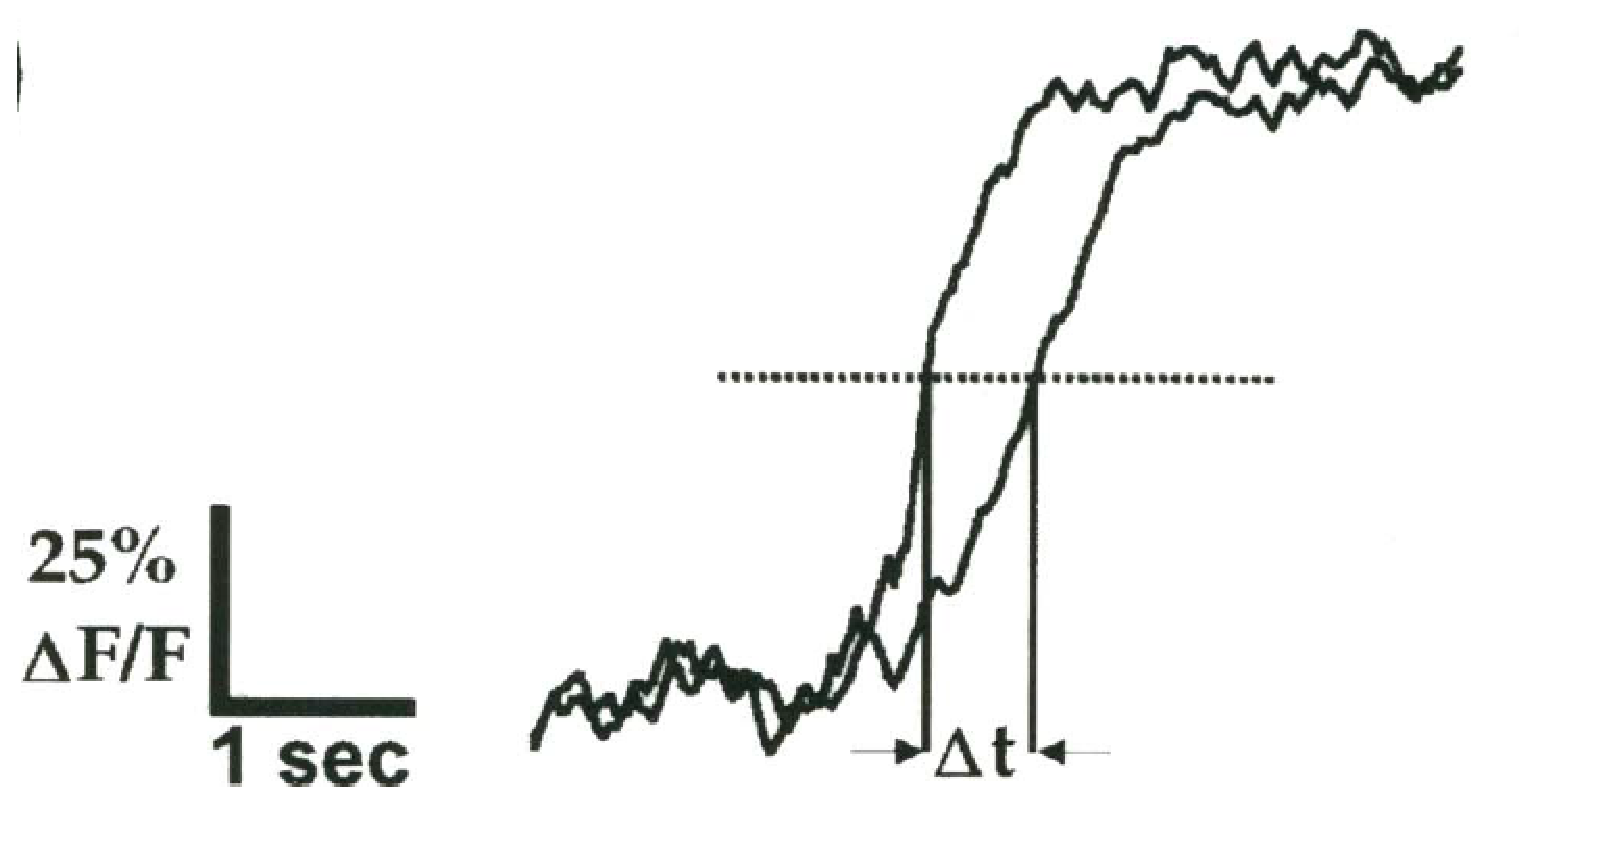
\includegraphics[height=5cm,
    angle=0]{./images/measure_Ca-waves.eps}}
\caption{How the speed of calcium wave is measured \citep{wang1993lpf}}
\label{fig:measure_Ca-wave}
\end{figure}


The length of the wavefront L was measured by calculating the distance in the
direction of propagation between the points where the fluorescence signal equals
10\% and 90\% of the maximum $\Delta F/F$.



\subsection{Calcium waves in cardiac cells}

The hormone endothelin-1 (ET-1) was used to to trigger the production of IP3.
\citep{domeier2008} pointed out that underlies the positive inotropic action of
endothelin-1 (ET-1) on ventricular myocytes, ET-1 provokes increase in [IP3]
concentration. As ET-1 is a potent vasoconstrictor hormone that have inotropic,
arrhythmic, and hypertrophic effects on cardiomyocytes, it's suggested that
IP3R-evoked $\Ca$ signals can occur. To prove that, they applied ET-1 to
electrically paced rabbit ventricular myocytes and actually it shows an increase
(38\%) in peak $\Ca$ transient, which is abolished by applying IP3R-antagonist.
Despite this convincing discovery, there are more questions regarding the
functional role of IP3R in the heart. However, the role of inotropy caused by
IP3R activation is generally modest in adult atrial and ventricular myocytes
compared with their proarrhythmic effect. 

Calcium waves released from nuclei mediated by IP3 was recently found in
neonatal cardiomyocyte \citep{luo2008}. IP3Rs were activated by
$\alpha_1$-adrenergic receptor ($\alpha_1$AR) stimulation or by IP3 application
(in saponin-permeabilized cell).  This can increase spark frequency around the
nucleus of neonatal rat ventricular myocytes. This gave to {\it nuclear $\Ca$
waves}. 

Interplay between IP3R and RyR2 were also found when testing neonatal (days 1-2)
and juvenile (days 8-10) \citep{janowski2010}. It's suggested that in developing
stage of cardiomyocyte, in addition to RyR-gated $\Ca$ signal, IP3-gated $\Ca$
release is also sufficiently large in magnitude and duration to trigger or
contribute to CICR and cardiac contraction. 

\section[Camacho et al. (1993)]{Camacho et al. (1993) - $\Ca$ waves in Xenopus
laevis oocytes}

\citep{camacho1993}

\section{Marchant et al. (1999,2001)}

\citep{marchant1999, marchant2001}


\section{aaa}

IP3-mediated Ca2+-release coupled to Ca2+-activated PLC can generate
oscillations, without any requirement of IP3R regulation by Ca2+ (26,27). These
models have been criticized because in some cell types Ca2+ oscillations can
also be elicited by IP3 or its nonmetabolizable analogs (3,28,29). The


\section{Ploti et al. (2006) - calcium oscillation}


Calcium oscillation is described in Sect.\ref{sec:calcium-oscill-waves}.
Here, the model of both [$\Ca$]c and IP3 level that accounts for both positive
and negative feedback on IP3 productions.
